\appendix
\chapter{Pilot Study Material}
\label{app:PilotStudyMaterial}
\section{Introduction to TDD}
Test-driven development is a new way to develop software. With TDD
developers \textit {(1) write new code only if an automated test has
failed; (2) eliminate duplication iteratively in software
development.} We will be implementing a stack data structure in TDD.
Please keep this in mind while you are participating this study. I
provided you with a quick reference \cite{TDDQuickReference} and the
rhythm of TDD \cite{TDDRhythm} to help you do TDD programming.
\subsection{TDD Quick Reference}

(Picture of Gunjan Doshi's TDD quick reference guide \cite{TDDQuickReference}.)

\subsection{Rhythm of TDD}

(Picture of Gunjan Doshi's TDD rhythm guide \cite{TDDRhythm}.)

\section{Stack Implementation in TDD}
I provide additional instructions for this pilot study. This section
includes description and instructive procedure to implement the stack
data structure in TDD. Stack works in Last-In-Last-Out (LILO)
principle. Its operations include
\textit{Push}, \textit{Pop}, \textit{Top}, and \textit{isEmpty}.
\begin{itemize}
\item The \textit{Push} function inserts an element onto the top of the \textit{Stack}.
\item The \textit{Pop} function removes the topmost element and returns it.  
\item The \textit{Top} function returns the topmost element but does not remove it from the \textit{Stack}.
\item The \textit{isEmpty} function returns true when there are no elements on the \textit{Stack}.
\end{itemize}

Note: some of this documentation are excerpted from \cite{Newkirk:04}.
\begin{enumerate}
\item \textbf{Test List (or TO-DO list)}

The first step is to brainstorm a list of tasks. The goal of this
activity is to create a task list from the requirements. Note that
this list does NOT have to be completed at beginning and you may
dynamically maintain it on the fly. Here is a task list example
maintained by Kent Beck in his book ``Test-Driven Development by
Example'' \cite{Beck:03}:
\begin{quote}
\$5 + 10 CHF = \$10 if rate is 2:1 \\
\sout{\$5 * 2 = \$10} \\
Make ``amount'' private \\
\sout{Dollar side-effects?} \\
Money rounding? \\
equals() \\
hashCode() \\
\end{quote}

Same as Beck did, you may work out a list of tasks for stack.
\begin{itemize}
\item {Create a \textit{Stack} and verify that \textit{isEmpty} is true.}
\item {\textit{Push} a single object on the \textit{Stack} and verify that \textit{isEmpty} returns false.}
\item {\textit{Push} a single object, \textit{Pop} the object, and verify that \textit{isEmpty} returns true.}
\item {\textit{Push} a single object, remembering what it is; \textit{Pop} the object, and verify that the two objects are equal.}
\item {\textit{Push} three objects, remembering what they are; \textit{Pop} each one, and verify that they are removed in the correct order.}
\item {\textit{Pop} a \textit{Stack} that has no elements.}
\item {\textit{Push} a single object and then call \textit{Top}. Verify that \textit{isEmpty} is false.}
\item {\textit{Push} a single object, remembering what it is; and then call \textit{Top}. Verify that the object returned is the same as the one that was pushed.}
\item {Call \textit{Top} on a \textit{Stack} with no elements.}
\end{itemize}

\item \textbf{Choose the First Test}

There is a list of tasks to start with. The philosophy of TDD is to
choose the simplest test that gets you started and solves a small
piece of the problem. The simplest one in the list is: ``Create a
Stack and verify that isEmpty is true.'' It is also an option to
choose a test that describes the essence of what you are trying to
accomplish. Using stack as an example, functions \textbf{Push} and
\textbf{Pop} are essential.

\item \textbf{Test 1: Create a {\em Stack} and verify that {\em isEmpty} is true.}

You start with a class called TestStack and add one assertion to check
whether isEmpty returns truth.
{\small\begin{verbatim}
  public void  testStackEmptiness() {
    Stack stack = new Stack();
    assertTrue("Test emptiness of Stack", stack.isEmpty());	
  }
\end{verbatim}}

This code will not compile because there is no Stack object created
yet. You should go ahead to implement Stack and provide
\textit{isEmpty()}. To make it simple you can just return constant
boolean value true in body of \textit{isEmpty()}.
{\small\begin{verbatim}
  public boolean isEmpty() {
    return true;
  }
\end{verbatim}}

\item {\textbf{Test 2: {\em Push} a single object on the stack and verify that {\em isEmpty} is false.}}

Remember to start with test first NOT to create push before you see
compilation error or test failure.
{\small\begin{verbatim}
  public void testPushOne() {	
    Stack stack = new Stack();
    stack.push("first element");
    assertFalse("Stack has one element, it is not empty", 
                stack.isEmpty());
  }
\end{verbatim}}

\item {\textbf{Test 3: {\em Push} a single object, {\em Pop} the object, and verify that {\em isEmpty} is true.}}

This test introduces a new method called Pop, which returns the
topmost element and removes it from the Stack.

{\small\begin{verbatim}
  public void testPop() {	
    Stack stack = new Stack();
    stack.push("first element");
    stack.pop();
    assertTrue("Stack has no element after pop",  stack.isEmpty());
  }
\end{verbatim}}

\item {\textbf{Test 4: {\em Push} a single object, remembering what it is; {\em Pop} the object, and verify that the two objects are equal.}}

{\small\begin{verbatim}
  public void testPushPopContent() {	
    Stack stack = new Stack();
    String value = "9001";
    stack.push(value);
    String result = (String) stack.pop();
    assertEquals("The popped up value equals to the pushed one", 
                 value, result);
  }
\end{verbatim}}

Please keep in mind that you don't have to have the correct
implementation to make test pass. You can always add a little, run the
test to see it fail, and rework until it passes the test.

\item {\textbf{Test 5: {\em Push} three objects, remembering what they are; {\em Pop} each one, and verify that they are correct.}}

In previous implementation you can simply have one element to make all
those tests pass. With this test you will very likely implement an
array, ArrayList, or vector to hold objects that are pushed onto the
stack.

\item {\textbf{Test 6: {\em Pop} a {\em Stack} that has no elements.}}

As you may work on Java for a while, exception should be thrown when
there is illegal operation like this one.
{\small\begin{verbatim}
  public void testPopEmptyStack() {
    try {
      stack.pop();
      fail("Exception is expected when pop value from empty stack"); 
    }
    catch (Exception e) {
      //Do nothing. Exception is expected.
    }  
  }
\end{verbatim}}

\item {\textbf{Test 7: {\em Push} a single object and then call {\em Top}. Verify that {\em isEmpty} returns false.}}

{\small\begin{verbatim}
  public void testPushTop() {
    Stack stack = new Stack();
    stack.push("42");
    stack.top();
    assertFalse("Stack is not empty after top() is called.", 
                stack.isEmpty());
  }
\end{verbatim}}

\item {\textbf{Test 8: {\em Push} a single object, remembering what it is; and then call {\em Top}.}}

Verify that the object returned is equal to the one that was pushed.

\item {\textbf{Test 9: {\em Push} multiple objects, remembering what they are; call {\em Top}, and verify that the last item pushed is equal to the one returned by {\em Top}.}}
\item {\textbf{Test 10: {\em Push} one object and call {\em Top} repeatedly, comparing what is returned to what was pushed.}}
\item {\textbf{Test 11: Call {\em Top} on a {\em Stack} that has no elements.}}
\item {\textbf{Test 12: {\em Push} null onto the {\em Stack} and verify that {\em isEmpty} is false.}}
\item {\textbf{Test 13: {\em Push} null onto the {\em Stack}, {\em Pop} the {\em Stack}, and verify that the value returned is null.}}
\item {\textbf{Test 14: {\em Push} null onto the {\em Stack}, call {\em Top}, and verify that the value returned is null.}}

\end{enumerate}

We don't have either instructional code in last 7 test cases. Stack
is a simple data structure and TDD does not have high technique
requirements you should be able to implement it and make all these
tests pass with small amount of effort.

\chapter{User Stories for Stack Data Structure}
\label{app:UserStoriesStack}

\clearpage
\begin{center}
\LARGE{\textbf{A Hands-on Practice of TDD: User Stories of Stack}}
\end{center}

\noindent The objective of this assignment is to practice TDD development with stack problem. User stories are provided to help you develop stack in TDD iteratively. Stack is a data structure that works in Last-In-First-Out principle. It includes four basic operations: Push, Pop, Top, and isEmpty. 
\begin{itemize}
\item The Push function inserts an integer element onto the top of the Stack.
\item The Pop function removes the topmost integer element and returns it.
\item The Top operation returns the topmost integer element but does not remove it from the Stack.
\item The isEmpty function returns truth when there are no elements on the Stack and false otherwise.
\end{itemize}

\noindent Please note that this assignment is not just about programming a stack data structure. Instead, it is a hands-on practice on Test-Driven Development. You should implement stack iteratively using the following user stories.\\

\noindent 1. Create a stack and verify that it is empty\\
\textbf{Requirement:} Be able to construct a stack which is empty initially. Verify that it is empty.\\

\noindent 2. Push an integer value and verify that stack is not empty. \\
\textbf{Requirement:} Push value 1001 onto the stack, check whether stack is not empty afterward.\\

\noindent 3. Push an integer value, pop it, and verify that stack is empty. \\
\textbf{Requirement:} Push value 1001 onto the stack, call pop, check to make sure that stack is empty.\\

\noindent 4. Push an integer value, remember what it is; pop a value from stack, verify that it is equal to the one pushed. \\
\textbf{Requirement:} Push value 1001 onto the stack, call pop, examine whether the popped value is 1001.\\

\noindent 5. Push three integer values, remember what they are; pop each one, and verify that they are correct. \\
\textbf{Requirement:} Push integer values 1001, 2001, 3001 onto the stack, call pop three times. It should return 3001, 2001 and 1001 respectively.\\

\noindent 6. Pop an integer value from stack that is empty. \\
\textbf{Requirement:} Exception StackEmptyException should be thrown when trying to pop a value from an empty stack.\\

\noindent 7. Push an integer value, call top, and verify that the returned value equal to the pushed value. \\
\textbf{Requirement:} Push value 1001 onto the stack, call top, the returned value should be  1001.\\

\noindent 8. Push three integer values, call top three times, and verify the returned values always equal to the last value. \\
\textbf{Requirement:} Push 1001, 2001, 3001 onto the stack, call top three times, and the returned values should be 3001.\\

\noindent 9. Push one integer value, call top repeatedly, comparing what is returned to what was pushed. \\
\textbf{Requirement:} Push 1001 onto the stack, call top three times, and the returned values should be 1001.\\

\noindent 10. Call top on a stack with no element. \\
\textbf{Requirement:} Exception StackEmptyException should be thrown when trying to top a value from an empty stack. 

\chapter{User Stories for Roman Numeral}
\label{app:UserStoriesRomanNumeral}

\clearpage
\begin{center}
\LARGE{\textbf{A Hands-on Practice of TDD: User Stories of Roman Numeral Conversion}}
\end{center}

Roman numerals are written as combinations of the seven letters in the
Table \ref{tab:AppRomanNumerals} (excerpted from URL 
http://www.yourdictionary.com/crossword/romanums.html).
\begin{table}[!h]
\centering
  \begin{tabular}{|p{2cm}|p{2cm}|}
  \hline
    I=1  & C=100  \\ \hline
    V=5  & D=500  \\ \hline
    X=10 & M=1000 \\ \hline
    L=50 &        \\ 
  \hline
  \end{tabular}
  \caption{Roman Numerals}\label{tab:AppRomanNumerals}  
\end{table}
If smaller numbers follow larger numbers, the numbers are added. If a
smaller number precedes a larger number, the smaller number is
subtracted from the larger. For example:
\begin{itemize}
\item VIII = 5 + 3 = 8
\item IX   = 10 - 1 = 9
\item XL   = 50 - 10 = 40
\end{itemize}

\begin{table}[!h]
\centering
  \begin{tabular}{|p{0.3cm}|p{1.2cm}||p{0.3cm}|p{1.2cm}||p{0.3cm}|p{1.2cm}||p{0.3cm}|p{1.2cm}||p{0.3cm}|p{1.2cm}|}
    \hline 1 & \textbf{I} & 11 & \textbf{XI} & 21 & \textbf{XXI} & 31
    & \textbf{XXXI} & 41 & \textbf{XLI} \\ \hline 2 & \textbf{II} & 12
    & \textbf{XII} & 22 & \textbf{XXII} & 32 & \textbf{XXXII} & 42 &
    \textbf{XLII} \\ \hline 3 & \textbf{III} & 13 & \textbf{XIII} & 23
    & \textbf{XXIII} & 33 & \textbf{XXXIII} & 43 & \textbf{XLIII} \\
    \hline 4 & \textbf{IV} & 14 & \textbf{XIV} & 24 & \textbf{XXIV} &
    34 & \textbf{XXXIV} & 44 & \textbf{XLIV} \\ \hline 5 & \textbf{V}
    & 15 & \textbf{XV} & 25 & \textbf{XXV} & 35 & \textbf{XXXV} & 45 &
    \textbf{XLV} \\ \hline 6 & \textbf{VI} & 16 & \textbf{XVI} & 26 &
    \textbf{XXVI} & 36 & \textbf{XXXVI} & 46 & \textbf{XLVI} \\ \hline
    7 & \textbf{VII} & 17 & \textbf{XVII} & 27 & \textbf{XXVII} & 37 &
    \textbf{XXXVII} & 47 & \textbf{XLVII} \\ \hline 8 & \textbf{VIII}
    & 18 & \textbf{XVIII} & 28 & \textbf{XXVIII} & 38 &
    \textbf{XXXVIII}& 48 & \textbf{XLVIII} \\ \hline 9 & \textbf{IX} &
    19 & \textbf{XIX} & 29 & \textbf{XXIX} & 39 & \textbf{XXXIX} & 49
    & \textbf{XLIX} \\ \hline 10 & \textbf{X} & 20 & \textbf{XX} & 30
    & \textbf{XXX} & 40 & \textbf{XL} & 50 & \textbf{L} \\ \hline
    \end{tabular} \caption{Roman Numerals Conversion Table}
    \label{tab:AppRomanNumeralTable}
\end{table}

Please note that this assignment is not just about programming a roman
numerals conversion. Instead, it is a hands-on practice on Test-Driven
Development. You should use the provided user stories to write test
case first, and let the tests to drive the code implementation. \\

\noindent \textbf{Roman Numeral Conversion User Stories}:
\begin{enumerate} 
  \item The conversion program returns empty string `` '' to value 0.
  \item Roman numeral is ``I'' to value 1.
  \item Roman numeral is ``II'' to value 2
  \item Roman numeral is ``III'' to value 3
  \item Roman numeral is ``IV'' to value 4, not "IIII"
  \item Roman numeral is ``V'' to value 5
  \item Roman numeral is ``VI'' to value 6
  \item Roman numeral is ``VIII'' to value 8
  \item Roman numeral is ``IX'' to value 9, not VIIII
  \item Roman numeral is ``X'' to value 10
  \item Roman numeral is ``XI'' to value 11
  \item Roman numeral is ``XV'' to value 15
  \item Roman numeral is ``XIX'' to value 19
  \item Roman numeral is ``XX'' to value 20
  \item Roman numeral is ``XXX'' to value 30 
\end{enumerate}

\chapter{Case Study Consent Form}
\label{app:CaseStudyConsentForm}

\begin{figure}[htbp]
  \centering
  \includegraphics[height=1.0\textheight]{figs/ExtendedConsentForm.eps}
\end{figure}

\chapter{User Stories for Bowling Score Keeper}
\label{app:UserStoriesBSK}
\clearpage
\begin{center}
\LARGE{\textbf{Test-Driven Development Exercise: Bowling Score Keeper}}
\end{center}

The objective is to develop an application that can calculate the score
of a SINGLE bowling game using TDD. There is no graphic user
interface. You work on objects and JUnit test cases only in this
assignment. We divide the bowling game requirements into a set of user
stories, which can serve as your to-do list. You should be able to
come up with a solution without much comprehension of the bowling game
rules. We encourage you to solve this programming task using TDD as much
as possible.

\noindent \textbf{1. Frame} \\
\textit{10 pins are arranged in an equilateral triangle in bowling game. It is called ``frame''. The goal of a frame is to knock all 10 pins down. The player has two chances, called ``throws'',  to do so.} \\
\textbf{Requirement:} Define frame so that it has two integer attribute values. Each value represents a throw. \\
\textbf{Example:} [2, 4] is a frame with two throws. Note that you don't have to check parameters.\\

\noindent \textbf{2. Frame Score} \\
\textit{The frame score is the sum of the first throw and second throw. For example, score of frame [3,5] is 8;  score of frame[0,0] is 0, which is called ``gutter'' in bowling game.  
} \\
\textbf{Requirement:} Compute score of a frame. \\
\textbf{Example:} The score of frame [2, 6]  is 8.  Frame [0, 9]'s score is 9. \\

\noindent \textbf{3. Game} \\
\textit{A single bowling game consists of 10 frames.} \\
\textbf{Requirement:} Define bowling game which consists of 10 frames. \\
\textbf{Example:} A sequence of frames  [1,5] [3,6] [7,2] [3,6] [4,4] [5,3] [3,3] [4, 5] [8, 1] [2, 6] is a game. Note that we will use this game many times from now on. We will modify only a few frames each time to represent different bowling game scenarios.\\

\noindent \textbf{4. Game Score} \\
\textit{The score of a bowling game is the sum of its 10 frames.} \\
\textbf{Requirement:} Compute the score of a bowling game. \\
\textbf{Example:} The score of above game is 81. \\

\noindent \textbf{5. Strike} \\
\textit{A frame is called ``strike'' if 10 pins are knocked down by the first throw. In this case, there is no second throw. A strike frame can be written as [10,0]. The score of  a strike is 10 plus the following two throws. Suppose there are consecutive frames such as [10, 0] and [3, 6], then the strike frame score will be 10 + 3 + 6 = 19.} \\
\textbf{Requirement:} Compute the score of a bowling game with a strike frame. \\
\textbf{Example:} Let's suppose the first throw in above game is a strike. The bowling game will have frames [10,0] [3,6] [7,2] [3,6] [4,4] [5,3] [3,3] [4, 5] [8, 1] [2, 6]. Its score will be 94.  
\\

\noindent \textbf{6. Spare} \\
\textit{A frame is called ``Spare'' when 10 pin are knocked down by two throws. For example, [1,9], [4,6], [7,3] are all spares. The score of a spare frame is 10 plus the next throw following it. If you have two frames [1,9] and [3,6] in a row, the spare frame score will be 10 + 3 = 13.} \\
\textbf{Requirement:} Compute the score of a bowling game with a spare frame. \\
\textbf{Example:} Similarly let's assume the first frame in above game is a spare [1,9], then it will have frames [1,9] [3,6] [7,2] [3,6] [4,4] [5,3] [3,3] [4, 5] [8, 1] [2, 6]. Its score will be 88. \\

\noindent \textbf{7. Strike and Spare} \\
\textit{A strike frames is followed by a spare frame. For example, [10,0], [4,6], [7, 2] are three consecutive frames with a strike followed by a spare. Score for the strike is 10 + 4 + 6 = 20, and score for the spare is 10 + 7 = 17.} \\
\textbf{Requirement:} Compute the score of a bowling game with a spare frame follows a strike. \\
\textbf{Example:} Similarly let's assume the first two frames are [10, 0] and [4, 6] in above game. The game will have frames [10,0] [4,6] [7,2] [3,6] [4,4] [5,3] [3,3] [4, 5] [8, 1] [2, 6]. Its score will be 103. \\

\noindent \textbf{8. Multiple Strikes} \\
\textit{Two strikes in a row is possible in a real bowling game. To three frames [10, 0], [10, 0] and [7,2], score for the first strike will be 10 + 10 + 7 = 27.  The second strike score will be 10 + 7 + 2 = 19.} \\
\textbf{Requirement:} Compute the score of a bowling game with two strikes in a row. \\
\textbf{Example:} Let's assume the first two frames are both strikes, then the bowling game will look like [10,0] [10,0] [7,2] [3,6] [4,4] [5,3] [3,3] [4, 5] [8, 1] [2, 6]. Its score will be 112.  \\

\noindent \textbf{9. Multiple Spares} \\
\textit{Two spares in a row is another case.} \\
\textbf{Requirement:} Compute the score of a bowling game with two spares in a row.\\
\textbf{Example:} Assuming the first two frames are spares, then the bowling game will look like [8,2] [5,5] [7,2] [3,6] [4,4] [5,3] [3,3] [4, 5] [8, 1] [2, 6]. The game score will be 98. \\

\noindent \textbf{10. Spare as the Last Frame} \\
\textit{When the last frame is a SPARE, the player will be given a bonus throw. However, this throw does not belong to a regular frame. It is only used to calculate the score of the last spare.} \\
\textbf{Requirement:} Compute the score of a bowling game when the last frame is a spare. \\
\textbf{Example:} Assuming the last frame is a spare in above game,  then game will be [1,5] [3,6] [7,2] [3,6] [4,4] [5,3] [3,3] [4, 5] [8, 1] [2, 8] with bonus throw [7]. Its score will be 90. \\

\noindent \textbf{11. Strike as the Last Frame} \\
\textit{When the last frame is a STRIKE, the player will be given two bonus throws. However, these two throws do not belong to a regular frame. They are used to calculate score of the last strike frame only.} \\
\textbf{Requirement:} Compute the score of a bowling game when the last frame is a strike. \\
\textbf{Example:} Assuming the last frame is a strike in above game,  it will be [1,5] [3,6] [7,2] [3,6] [4,4] [5,3] [3,3] [4, 5] [8, 1] [10, 0] with bonus throws [7, 2]. The game score will be 92. \\

\noindent \textbf{12. Bonus is a strike} \\
\textit{Bonus strike will not be counted as strike in a bowling game.} \\
\textbf{Requirement:} Assuming the last frame is a spare and the bonus is a strike, compute the score of this game.\\
\textbf{Example:} Assuming the last frame is a spare and the bonus is a strike in above game,  the game will be [1,5] [3,6] [7,2] [3,6] [4,4] [5,3] [3,3] [4,5] [8,1] [2,8] with bonus throw [10, 0]. The game score will be 93. \\

\noindent \textbf{13. Best Score} \\
\textit{} \\
\textbf{Requirement:} Compute the score of the bowling game when all frames are strikes.\\
\textbf{Example:} Assuming all frames are strikes including bonus. The game looks like [10,0] [10,0] [10,0] [10,0] [10,0] [10,0] [10,0] [10,0] [10,0] [10,0] with bonus throws [10,10]. It is a perfect game and the game score is 300. \\

\noindent \textbf{14. A Real Game} \\
\textit{} \\
\textbf{Requirement:} To a game with frames [6,3] [7,1] [8,2] [7,2] [10,0] [6,2] [7,3] [10,0] [8,0] [7,3] [10], its score is 135.  

\chapter{Participant Interview Guideline in Case Study}
\label{app:CaseStudyInterviewGuide}

\noindent \textbf{Purpose} \\
The purpose of this interview is to gather participants' experience of
TDD including how they think about TDD, whether and how TDD affects
their software development, whether can Zorro help them, and how Zorro
can be used? The protocol of the interview is described here.\\

\noindent \textbf{Interviewer} \\
Hongbing Kou \\

\noindent \textbf{Interviewees} \\
Participants of the Zorro case study \\

\noindent \textbf{Time and place}\\ 
Participants will be interviewed by me in the lab after they finish
validating Zorro's inference on their behaviors. The interview will
last from 15 to 20 minutes.  \\

\noindent \textbf{Facility}\\ 
Notepad, pen, and tape recorder. I will ask interviewee's permission for
the use of tape recorder. \\

\noindent \textbf{Outline}
\begin{itemize}
  \item {Questions from the participant}
  \item {Experiences and opinions on unit testing and Test-Driven Development}
  \item {Opinions on TDD measurement with Zorro. In what way does the measurement tool help?}
  \item {Zorro usefulness evaluation}
  \item {Possible improvements of Zorro}
\end{itemize}

\noindent \textbf{List of interview questions}
\begin{enumerate}
\item {Questions from the participants}

I will give interviewees some time at the beginning to ask me
questions. They may ask questions about TDD, Zorro or this
study. Purpose of this is to let participants feel comfortable before
the interview starts. This may lead them to get involved and start
talking.

\item {Unit testing and Test-Driven Development}

\begin{itemize}
  \item {When and where did you learn unit testing?}
  \item {How do you apply unit testing in your software development?} 
  
  Do you write testing code when you are not confident about a program? \\
  Do you write testing code after you finish a program? \\
  Do you write testing code when you want to improve your testing coverage? \\
  Did you ever write testing code first before you learned TDD?
  
  \item {How much testing code do you write?}

  How much is the code coverage of the programs you wrote in the software engineering class? \\
  Can you comment on the use of unit testing in software development?
  
  \item {Can you compare TDD to the testing strategy you did before?}
  
  How do you think of TDD? Is it helpful to improve software quality? \\ 
  How comfortable it is for you to do TDD programming?
  What problems you have when you programmed in TDD?
\end{itemize} 
 
\item {Please use scale 1 to 5 to assess the usefulness of Zorro's TDD analyses (1 stands for least useful and 5 stands for most useful). I would like you to justify your answers.}
    \begin{itemize}
      \item{Episode Inference}            
      \item{TDD Episode Demography}
      \item{TDD Episode Duration Distribution's}
      \item{Test Effort vs. Production Effort}
      \item{Test Size vs. Production Size}
    \end{itemize}
\item {What other information you wish to have about TDD development?}
  
  How about an Eclipse plug-in indicating whether you are doing TDD? \\
  How about an analysis showing your TDD performance over the time? \\
\end{enumerate}

\chapter{Participant Selections of TDD Analysis Usefulness Areas}
\label{app:UsefulnessAreas}
\begin{table}[!htbp]
\centering
  \begin{tabular}{|l|l|l|l|l|l|l|l|l|l|l|l|}
  \hline 
TDD Analysis   &   Useful Areas    &  A	&  K	&  L	&  N	&  O	&  P	&  Q	&  R	&  S	&  T  \\ \hline
    &  UA-1 &  X  &     &  X  &  X  &  X  &  X  &  X  &     &  X  &  X  \\ \cline{2-12}
    &  UA-2 &     &  X  &     &  X  &     &  X  &  X  &  X  &  X  &  X  \\ \cline{2-12}
    &  UA-3 &     &     &  X  &     &     &     &     &  X  &     &  X  \\ \cline{2-12}
    &  UA-4 &     &     &     &  X  &  X  &  X  &  X  &     &     &     \\ \cline{2-12}
    &  UA-5 &     &  X  &     &     &     &     &     &  X  &     &  X  \\ \cline{2-12}
    &  UA-6 &     &     &     &     &     &  X  &     &     &     &  X  \\ \cline{2-12}
    &  UA-7 &     &  X  &     &     &     &  X  &     &     &     &     \\ \cline{2-12}
\raisebox{10ex}[0pt]{Episode Demography}     
    &  UA-8 &     &     &  X  &  X  &  X  &  X  &  X  &     &     &  X  \\ \hline
    
    &  UA-1 &  X  &     &  X  &  X  &  X  &  X  &  X  &  X  &  X  &  X  \\ \cline{2-12} 
    &  UA-2 &     &     &     &     &     &  X  &     &     &  X  &  X  \\ \cline{2-12} 
    &  UA-3 &     &     &     &     &     &     &     &     &     &  X  \\ \cline{2-12} 
    &  UA-4 &  X  &     &  X  &  X  &  X  &     &  X  &     &  X  &  X  \\ \cline{2-12} 
    &  UA-5 &     &     &     &     &  X  &     &     &     &     &  X  \\ \cline{2-12}  
    &  UA-6 &     &     &     &     &     &  X  &     &     &     &  X  \\ \cline{2-12} 
    &  UA-7 &     &     &     &  X  &     &  X  &     &     &     &     \\ \cline{2-12} 
\raisebox{10ex}[0pt]{T/P Effort Ratio}  
    &  UA-8 &  X  &     &     &  X  &  X  &  X  &  X  &  X  &  X  &     \\ \hline

        &  UA-1 &  X  &     &  X  &     &  X  &  X  &     &  X  &  X  &     \\ \cline{2-12} 
    &  UA-2 &  X  &     &     &     &     &  X  &     &     &  X  &  X  \\ \cline{2-12} 
    &  UA-3 &     &     &     &  X  &     &     &     &     &     &  X  \\ \cline{2-12}  
    &  UA-4 &     &  X  &  X  &     &     &  X  &     &     &     &  X  \\ \cline{2-12} 
    &  UA-5 &     &     &     &     &     &     &     &  X  &     &     \\ \cline{2-12} 
    &  UA-6 &  X  &     &     &     &     &  X  &     &     &     &     \\ \cline{2-12} 
    &  UA-7 &     &     &     &     &     &  X  &     &     &     &     \\ \cline{2-12} 
\raisebox{10ex}[0pt]{T/P Size Ratio}  
    &  UA-8 &  X  &     &     &  X  &  X  &  X  &  X  &     &  X  &     \\ \hline
    
    &  UA-1 &  X  &     &  X  &     &  X  &  X  &  X  &  X  &  X  &     \\ \cline{2-12}   
    &  UA-2 &  X  &     &     &     &     &  X  &     &     &  X  &     \\ \cline{2-12} 
    &  UA-3 &     &     &  X  &     &     &     &     &     &     &     \\ \cline{2-12}    
    &  UA-4 &  X  &  X  &  X  &  X  &     &  X  &  X  &     &  X  &     \\ \cline{2-12} 
    &  UA-5 &     &     &     &     &     &     &     &     &     &     \\ \cline{2-12}    
    &  UA-6 &     &     &     &     &  X  &     &     &     &     &     \\ \cline{2-12} 
    &  UA-7 &     &     &     &     &  X  &     &     &     &     &     \\ \cline{2-12} 
\raisebox{10ex}[0pt]{Episode Duration}  
    &  UA-8 &     &     &     &     &     &     &     &  X  &     &     \\ \hline
    
    &  UA-1 &  X  &     &  X  &     &     &     &  X  &  X  &  X  &  X  \\ \cline{2-12} 
    &  UA-2 &  X  &     &     &  X  &     &  X  &     &  X  &  X  &  X  \\ \cline{2-12} 
    &  UA-3 &     &     &     &     &  X  &     &     &     &     &  X  \\ \cline{2-12}  
    &  UA-4 &     &  X  &  X  &     &  X  &     &  X  &     &     &  X  \\ \cline{2-12} 
    &  UA-5 &     &     &     &     &  X  &     &     &     &     &  X  \\ \cline{2-12}  
    &  UA-6 &  X  &     &  X  &     &     &     &     &     &     &  X  \\ \cline{2-12} 
    &  UA-7 &     &     &     &     &     &     &     &     &     &     \\ \cline{2-12}  
\raisebox{10ex}[0pt]{Duration  Distribution}  
    &  UA-8 &     &     &  X  &     &  X  &  X  &     &     &     &     \\ \hline
    \end{tabular}
  \caption{TDD Analysis Useful Areas}\label{tab:UsefulnessArea}  
\end{table}

